\documentclass{article}
\usepackage[a4paper, portrait, margin=1cm, right=1cm]{geometry}
\usepackage{fontspec}
\usepackage[fleqn]{amsmath}
\usepackage{setspace}
\usepackage{graphicx}

\graphicspath{./graphics/}
\setmainfont[Ligatures=TeX]{Linux Libertine}

\title{Информационные технологии. Лекция 04. Сенсорные системы}
\author{Студент группы 2305 Макурин Александр}
\date{06 марта 2023}

\begin{document}
\maketitle
\begin{sloppypar}
    Датчик — устройство, преобразающее контролируемую величину в удобную для обработки форму (из внешней среды в данные).

    Характеристики измерений:
    \begin{itemize}
        \item Чистота
        \item Качество
        \item Точность
    \end{itemize}

    Виды датчиков:
    \begin{enumerate}
        \item Направленные на измерение внутреннего состояния (e.g. датчик заряда аккумулятора)
        \item Физико-химический анализ окружающей среды (e.g. фоторезистор)
        \item Общая картина окружающей среды (e.g. видеорегистратор)
    \end{enumerate}

    Проблемы датчиков:
    \begin{itemize}
        \item Шумы
        \item Объединение нескольких измерений
    \end{itemize}

    \subsection*{Энкодеры}
    \begin{itemize}
        \item Абсолютные
        \item Накапливающие
    \end{itemize}

    Проблема (из-за окружающей среды) — локальный разброс. Даже при условии, что в среднем движение не отклоняется от модели (называется нулевым средним), то в процессе прохождения маршрута из-за внешних факторов может произойти отклонение на одной из частей маршрута и финальная точка вообще не будет достигнута.

    Калибровка, в среднем, приводит к нужному результату, но смотри пункт выше.

    Как было рассмотрено в прошлой лекции, системы навигации делятся на глобальные и локальные.

    \section{Локальные системы навигации}
    От некоторого объекта — навигация за счёт информации о расстоянии до некоторого объекта, местоположение которого известно.
    \subsection{Собственные}
    Собственные — навигация за счёт информации о собственном перемещении. E.g. отслеживание количества поворотов каждого колеса посредством энкодеров и на основе этих данных определять поворот и отклонение относительно начальной точки.

    $r = f(r_0, \upsilon, \theta) + \varepsilon$, где $r$ - перемещение, $r_0$ - начальное положение, $\upsilon$ - скорость, $\theta$ - угол.
    При этом при росте перемещения, т. е. чем дольше происходит передвижение, увеличивается общая погрешность.
    \begin{center}
        \begin{tabular}{ |c|c|c| }
            \hline
            $f, e, g$ — погрешности                        & Движение без «шума»                & Движение с «шумом» \\
            \hline
            Движение по прямой                             & $\begin{pmatrix}
                                                                      x_{new} \\ y_{new} \\ \theta_{new}
                                                                  \end{pmatrix} =
            \begin{pmatrix}
                    x + D\cos \theta \\ y + D\sin \theta \\ \theta
                \end{pmatrix}$ &
            $\begin{pmatrix}
                     x_{new} \\ y_{new} \\ \theta_{new}
                 \end{pmatrix} =
                \begin{pmatrix}
                    x + (D + e)\cos \theta \\ y + (D + e)\sin \theta \\ \theta + f
                \end{pmatrix}
            $
            \\
            \hline
            Поворот                                        & $\begin{pmatrix}
                                                                      x_{new} \\ y_{new} \\ \theta_{new}
                                                                  \end{pmatrix} =
            \begin{pmatrix}
                    x \\ y\\ \theta + \alpha
                \end{pmatrix}$                       &
            $\begin{pmatrix}
                     x_{new} \\ y_{new} \\ \theta_{new}
                 \end{pmatrix} =
                \begin{pmatrix}
                    x \\ y \\ \theta + \alpha + g
                \end{pmatrix}
            $
            \\
            \hline
        \end{tabular}
    \end{center}

    \subsubsection{Как использовать?}
    \begin{itemize}
        \item Совмещение с дополнительной информацией о роботе и/или
              окружающей среде
        \item Проприоцептивные — показывают внутреннее состояние системы.
        \item Проприоцептивные датчики (например, моторные энкодеры или
              датчики силовых воздействий) улучшают восприятие роботом
              собственного внутреннего состояния и движения.
        \item Без датчиков внешней среды робот движется вслепую.
        \item Распознавание мест и объектов, которые уже встречались ранее.
        \item Планирование движения в свободном пространстве для того, чтобы избежать
              столкновений с препятствиями.
        \item Взаимодействие с предметами и людьми.
        \item Создание общего представления об окружающей робота среде.
    \end{itemize}

    \subsubsection{Проприоцептивные датчики}
    \begin{itemize}
        \item Результаты измерений зависят только от состояния робота: $z = z(a)$
        \item Для передвижения на плоскости: $a = \begin{pmatrix} x \\ y \\ \theta \end{pmatrix}$
        \item Проприоцептивные измерения могут зависеть не только от текущего состояния, а и от предыдущих состояний или текущей скорости изменения состояния
    \end{itemize}
    \subsubsection{Датчики анализа внешней среды}
    \begin{itemize}
        \item Результаты измерений зависят от состояния робота и от состояния окружающей
              среды:
              $z = z(a, e)$
        \item Для передвижения на плоскости:
              $𝑎 = \begin{pmatrix}x \\ y \\ \theta \end{pmatrix}$
        \item Внешний мир: $e = <e_1, ..., e_n>$

              $e_i = \begin{pmatrix}x_i \\ y_i\end{pmatrix}$
        \item Состояние внешнего мира может быть параметризовано различными способами -
              например, списком координат стен или ориентиров.
        \item Состояние может быть либо неопределенным, либо полностью известным.
    \end{itemize}

    \subsubsection{Вероятностные датчики}
    \begin{itemize}
        \item Измерения являются неопределёнными. Измерения датчиков носят вероятностный характер.
        \item Для корректировки и прогноза требуется смоделировать вероятностный характер измерений.
        \item Описывается функцией правдоподобия.
        \item Вероятностный характер движения и измерения не позволяет использовать машинное обучение в полной мере.
    \end{itemize}

    \section{Объединение модели измерений и движений}
    \subsection{При собственной системе навигации}
    Используется локализация для калибровки. Для каждой точки пространства определяется вес $V_{\cdot}$ так, что $\sum V_\cdot = 1$. Тогда алгоритм локализации:
    \begin{enumerate}
        \item Предсказание движения, основанное на проприоцептивных датчиках.
        \item Обновление измерений, основанное на датчиках внешней среды.
        \item Нормализация
        \item Повторная выборка
    \end{enumerate}

    \subsubsection{Изначальная инициализация}
    В случае существования глобальной системы навигации (ГНС) мы сразу можем определить своё (робота) местоположение относительно выбранной точки (обычно вход в замкнутое пространство).

    В случае отсутвия ГНС применяется принцип суперпозиции — область примерного местоположение робота вычисляется на основании первых данных, в последствии с ростом получаемых данных от окружающей среды местоположение становится точнее (область примерного местоположения уменьшается).

    \subsubsection{Функция правдоподобия}
    Функция правдоподобия говорит, какова вероятность получения измерения z датчиком, учитывая, что истинное ожидаемое значение m. Т. е. насколько датчик ошибается при тех или иных входных данных.

    \subsection{SLAM}
    SLAM — simultaneous localization and mapping — одновременная локализация и построение карты.

    Задача SLAM — понять местоположение и нарисовать карту. Для этого есть 3 этапа:
    \begin{enumerate}
        \item Исследование окружения
        \item Построение модели окружения и окружающих объектов
        \item Навигация по построенному пространству
    \end{enumerate}

    \subsubsection{Групповая навигация SLAM}
    \begin{itemize}
        \item О глобальной системе координат объекты знают мало
        \item Задача — построить для всех субъективно-объективную глобальную систему координат в рамках e1 и e2.
              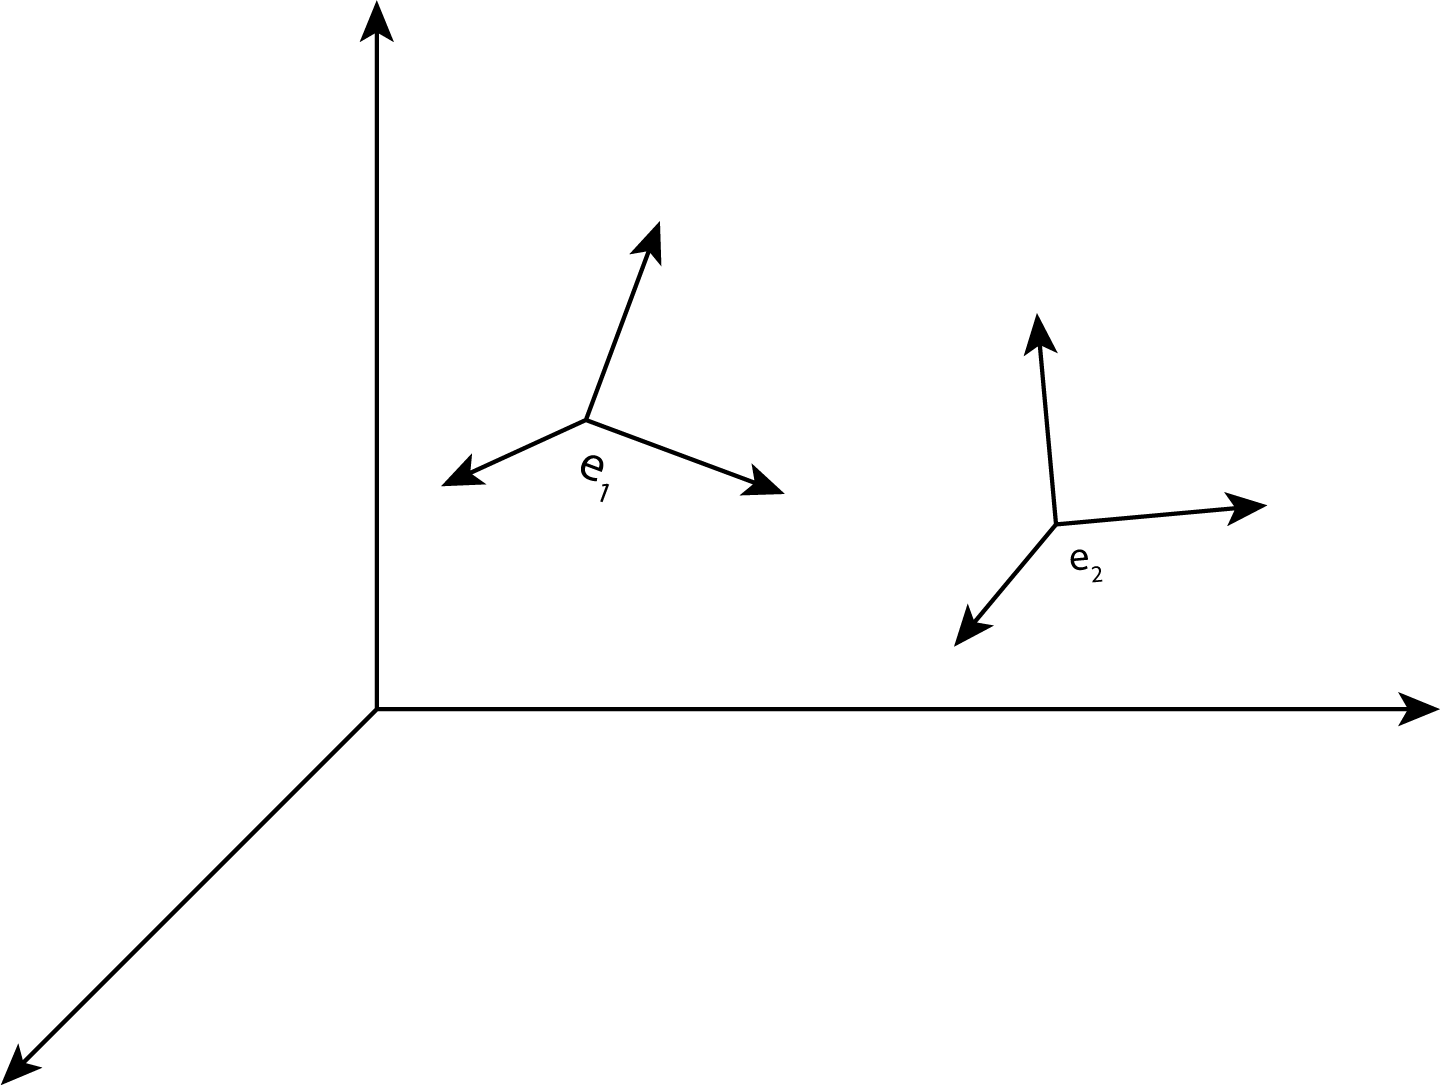
\includegraphics[width=0.6\textwidth]{graphics/SLAM.png}
    \end{itemize}

    \subsubsection{Сревнение с объектами}

    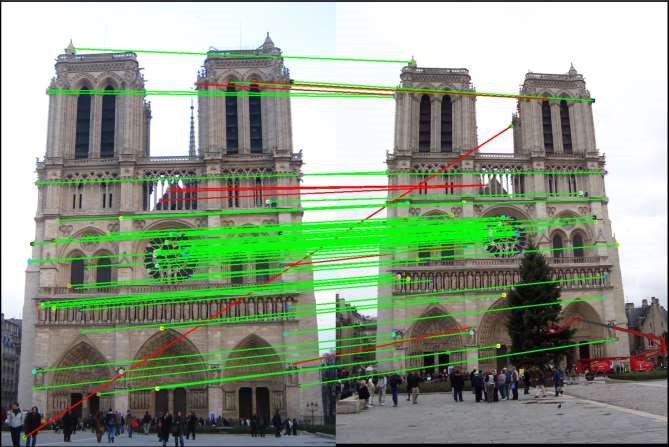
\includegraphics[width=\textwidth]{graphics/сравнение_с_объектами.png}

    Для точек с наибольшим градиентом строятся реперные точки.

    Решением задачи SLAM'а является сравнение нескольких матриц, разных во времени/пространстве.


    %TODO%
\end{sloppypar}
\end{document}